\documentclass{article}
\usepackage[T1]{fontenc}
\usepackage{lmodern}
\usepackage{graphicx}
\usepackage{amsmath,amssymb}
\usepackage[a4paper,margin=2cm]{geometry}
\usepackage[absolute,overlay]{textpos}
\setlength{\TPHorizModule}{1mm}
\setlength{\TPVertModule}{1mm}
\usepackage[indonesian]{babel}
\usepackage{hyperref}
\setlength{\emergencystretch}{2em}
% unit: Halaman 40

\begin{document}

% === Halaman 40 (python/native) ===

• Dari Gambar tersebut dapat dilihat bahwa:


Ci = Pi  Ek (Ci – 1 )


Pi = Ci  Dk (Ci – 1 )


   yang dalam hal ini, C0 = IV.

• Kesalahan 1-bit pada suatu blok plainteks tertentu akan merambat 

pada blok cipherteks yang berkoresponden dan blok-blok cipherteks 

selanjutnya pada proses enkripsi. 

40

(a) Enkripsi

% deskripsi: gambar native xref 169
\noindent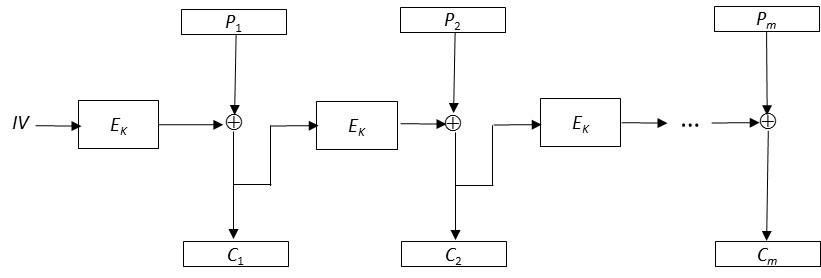
\includegraphics[width=0.85\textwidth]{../../images/python/page_040_img_01.jpeg}

\end{document}
